\section{Introduction}

Web users increasingly reach information through systems that decide what to retrieve before the user ever sees it. Search engines and recommender systems have long mediated this access; retrieval-augmented generation and emerging agentic interfaces add further layers that depend on an initial selection of Web content. This makes retrieval visibility a consequential system property. Ideally, semantically equivalent information should receive comparable opportunities to be discovered: relevance should determine what becomes visible, rather than arbitrary choices in how the same information is represented.

That expectation is difficult to guarantee for structured and semi-structured Web content. Products, jobs, hotels, restaurants, events, and profiles are commonly stored as fields and attribute-value records. Neural retrieval pipelines often flatten those records into text because Transformer encoders consume ordered token sequences. Many underlying facts, however, have no meaningful linear order. A hotel remains pet-friendly whether that field precedes or follows its parking policy. Once such records are serialized, position and contextual interaction can turn an implementation detail---a template, export order, or serializer---into an unintended retrieval signal. This raises a general Web robustness question: \emph{should semantically equivalent content receive substantially different visibility simply because it is represented differently?}

E-commerce offers a clean testbed for this question. Product attributes such as color, material, dimensions, style, and compatibility are naturally set-like. Their order can be permuted while product identity, semantic content, and human-assessed query relevance remain fixed. We can therefore intervene on representation without asking a model to rewrite, summarize, or add facts. In our controlled comparison, the product is the same, the facts are the same, the query and catalog are the same, and the retrieval model is the same; only the order used to serialize product attributes changes.

Figure~\ref{fig:example} makes the consequence concrete. For the query \emph{turquoise chair}, WANDS judges the product Exact-relevant. With all competitors fixed in their original representations, MiniLM ranks the target 5th under one attribute permutation and 1,527th under another. The underlying title and attribute-value multiset are identical. One representation is visible in a top-20 result set, while the other is effectively absent. Why should a serialization choice determine whether the same relevant product can be found?

\begin{figure}[H]
  \centering
  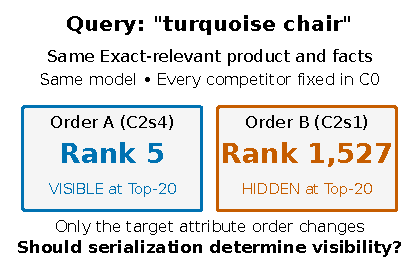
\includegraphics[width=\columnwidth]{figures/figure1_target_only.pdf}
  \Description{Two serializations of the same Exact-relevant turquoise chair contain identical facts and differ only in attribute order. Every competitor stays in C0. MiniLM ranks the target fifth and 1527th.}
  \caption{Target-only intervention: same product, facts, competitors, query, and model. Only the target attribute order changes, moving it from rank 5 to 1,527. All competitors remain in C0; this differs from catalog-wide permutations.}
  \label{fig:example}
\end{figure}

This is more than an embedding-space curiosity. Retrieval systems expose content through operational boundaries: a result page, a recommendation slate, or a candidate pool passed to a later ranker. A score change matters when it moves a relevant item across such a boundary. If a first-stage retriever excludes the item, a stronger reranker or downstream agent never receives it. Representation sensitivity can thus propagate through a Web retrieval pipeline even when average ranking quality changes little.

Existing product-retrieval research improves lexical, neural, and hybrid matching while usually treating the supplied catalog representation as fixed. Work on generative engine optimization (GEO) instead asks how creators can modify content to gain visibility; e-commerce GEO extends that optimization objective to product descriptions. Our question is prior to strategic optimization: why should fact-equivalent content receive different visibility at all? Recent work on tabular retrieval establishes that alternative serializations can change neural retrieval behavior. We extend this representation-robustness question to item-level product discovery, human relevance, practical cutoffs, candidate-generation loss, and a relevance-aware mitigation.

We study four research questions. \textbf{RQ1} asks whether representation alters product visibility across retriever families and product-search benchmarks. \textbf{RQ2} asks whether human-relevant products are materially affected, including under direct single-product interventions. \textbf{RQ3} asks whether a later cross-encoder can repair the instability or whether first-stage retrieval creates irrecoverable omissions. \textbf{RQ4} asks whether an order-invariant representation can improve robustness without a confirmed loss of retrieval effectiveness.

The paper makes four contributions:
\begin{itemize}
  \item \textbf{Problem formulation.} We formalize \emph{representation-induced visibility instability} and connect it to \emph{relevance--visibility alignment}: semantically irrelevant representation changes should not decide which relevant items cross a retrieval boundary.
  \item \textbf{Empirical evidence.} Across two public product-search benchmarks, three general-purpose neural retrievers, and an e-commerce-specific encoder, fact-equivalent attribute orders materially change the Top-$K$ visibility of human-relevant products.
  \item \textbf{Pipeline consequence.} We show that reranking reduces instability among surviving candidates but cannot repair serialization-induced candidate loss.
  \item \textbf{Mitigation.} We evaluate a simple permutation-invariant set representation that eliminates measured order sensitivity while producing a small, statistically inconclusive effectiveness change.
\end{itemize}
